\chapter{IoT Device Management}
In Zukunft ist eine stark ansteigende Anzahl an IoT Devices zu erwarten. Laut der International Data Corporation (IDC) dürften im Jahre 2020 in etwa 30 Milliarden Devices weltweit verbunden sein \cite{IDC15}. Unternehmen könnten potenziell mehrere Tausend Sensoren für ihre Zwecke einsetzen. Bereits bei herkömmlichen Computersystemen und Servern stellt das Management eine grosse Herausforderung dar. IoT Devices dürften potenziell in einer sehr viel grösseren Anzahl verbreitet sein als herkömmliche Geräte. Herausforderungen wie die Heterogenität, Verteilung und Security verschärfen sich mit der stetig wachsenden Anzahl an Geräten. 

IoT Devices durchleben in ihrem Lebenszyklus verschiedene Stadien. Ein Device Management Tool soll die Administration in jeder dieser Phasen Unterstützen.
\section{Device Lifecycle}
Der Lebenszyklus eines IoT Devices könnte beispielsweise aus folgenden fünf Phasen bestehen.
\begin{figure}[H]
\centering
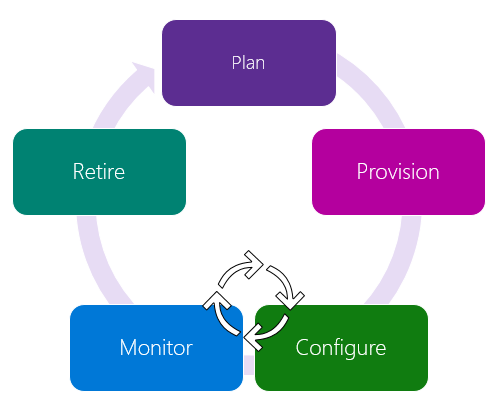
\includegraphics[scale=0.5]{images/hubdevmgmt-azure.png}
\caption{IoT Management Azure \cite{IoTMgmtAzure}}
\end{figure}
\subsubsection{Plan}
In der Planungsphase möchte man aufgrund von vorliegenden Daten eine Veränderung am System vornehmen. Um fundierte Entscheide in der Planungsphase zu ermöglichen werden Daten und Messwerte von Devices benötigt. Je einfacher diese Daten zugänglich-, respektive abfragbar sind, desto qualitativ hochwertiger und exakter kann geplant werden.
\subsubsection{Provision}
Neue Geräte müssen vor der produktiven Nutzung bereitgestellt werden. Dieser Prozess kann mehrere Personen und Aufgaben involvieren. Grundsätzlich werden neue Geräte in ein bestehendes System eingebunden oder ein komplett neues System aufgebaut.
\subsubsection{Configure}
Damit ein Device in den vorgesehenen Zustand versetzt werden kann benötigt es eine Konfiguration. Bei einer grossen Anzahl Devices empfiehlt es sich diesen Prozess bestmöglichst zu automatisieren. Dazu müssen alle Beteiligten  
\subsubsection{Monitor}
In der Monitoringphase sollen die Zustände der Devices überwacht werden. Ziel ist es, die Funktionalität und Korrektheit des angestrebten Verhalten sicherzustellen. Dies wird mittels periodischer Abfragen oder Observations sichergestellt. 
\subsubsection{Retire}
Am Ende des Lebenszyklus sollen Geräte geordnet aus dem System entfernt werden. Dabei gilt es den Prozess bestmöglich zu automatisieren und allfällige Vorschriften betreffend Datensicherheit und Datenschutz zu beachten. Andere Systeme wie das Inventar könnten ebenfalls in diesem Prozess beteiligt sein.
\section{Device Management Aufgaben}
\subsection{Provisionierung und Authentisierung}
Bevor neue Devices produktiv genutzt werden können, müssen sie entweder manuell, oder automatisch provisioniert werden. Beim Device Provisioning muss ein Gerät in einen Zustand gebracht werden, in dem es für eine oder mehrere vorgesehene Personen erreichbar respektive verfügbar ist.

\paragraph{Notwendige Schritte}So unterschiedlich die Geräte im Netzwerk und Internet auch sein können, so haben sie abstrakt gesehen die selben Schritte zu durchlaufen um für die produktive Nutzung Verfügbar zu werden:
\begin{itemize}
\item ein Device muss physisch am vorgesehenen Ort platziert werden,
\item die Stromversorgung (Stromnetz, Batterie, Akku) für das Gerät muss sichergestellt werden
\item das Device muss gestartet werden
\item eine Initialkonfiguration muss geladen werden
\item die Netzwerk- respektive Internetverbindung muss hergestellt werden
\end{itemize}
Ab dem Zeitpunkt der Erreichbarkeit des Netzwerks unterscheiden sich manuelles und automatisches Provisioning. Beim manuellen Provisioning greift der User oder Administrator entweder direkt über ein grafisches User Interface auf das Gerät zu und nimmt weitere Einstellungen vor oder er verbindet sich über das Netzwerk auf eine Benutzeroberfläche des Geräts. Beim automatischen Provisioning meldet sich das Device über das Netzwerk an einem Controller respektive einer Management Instanz.

\paragraph{Authentisierung} Bei einem Eintritt in ein bestehendes System, in diesem Falle die Bereitstellung eines neuen Devices, muss sich das Gerät am System authentisieren. Aus Sicherheitsgründen möchte man sicherstellen, dass die Zugriffe in das System kontrolliert werden. Es gibt verschiedene Möglichkeiten der Authentisierung:
\begin{itemize}
\item Authentisierung durch Wissen (z.B. Passwort, PIN, Challenge)
\item Authentisierung durch Besitz (z.B. RFID-Chip, Zertifikat, One Time Pin)
\item Authentisierung durch biometrische Merkmale (z.B. Fingerprint, Handvene)
\end{itemize}
Nicht alle Verfahren eignen sich für die Authentisierung von Devices. Ein Gerät selbst verfügt über keine biometrischen Merkmale, höchstens der Benutzer, welcher versucht das Gerät bereitzustellen. Ein Shared Secret in Form eines Passworts oder eine Chain-of-Trust mit Zertifikaten eignen sich für die Device Authentisierung gut. 

\paragraph{IoT Provisioning} IoT Devices sollten vor der produktiven Nutzung in einem definierten Prozess bereitgestellt werden. In einem ersten Schritt muss ein Device mit einem Netzwerk verbunden werden. Es ist weitgehend bekannt, dass eine grosse Vielfalt an Devices existieren. Manche von ihnen enthalten ein einfaches User Interface, andere nicht. So unterscheidet sich das Ausrollen von IoT Geräten von herkömmlichen PC's und Laptops indem man nicht direkt über das geräteeigene UI Einstellungen vornehmen kann.  

Ein neues IoT Device im System kontaktiert entweder seinen lokalen Gateway oder direkt einen Server über TCP/IP. Das System kann nun das neue Device aufnehmen und weitere Aufgaben wie beispielsweise das Laden der Konfiguration oder das Speichern von Geräteinformationen veranlassen. Netzwerke mit IoT Devices sind sehr dynamisch. Es werden häufig neue Teilnehmer aufgenommen oder alte Teilnehmer entfernt. Tools, welche diese Prozesse automatisieren sind stark gefragt. Devices sollen sich selbständig an Netzwerken anmelden können und sich bei zuständigen Servern für weitere Anweisungen registrieren. Solche Discovery Mechanismen sind für zukünftige Anwendungen essentiell \cite{IoTDiscovery10}.

Mit dem Prozess der automatischen Registrierung an Netzwerken und Systemen sind Fragen der Sicherheit verbunden. Man möchte selbstverständlich die Zugriffe in Netzwerke und Systeme korrekt authentisieren und autorisieren. Sicheres Bootstrapping von IoT Devices umfasst neben Authentisierung und Autorisierung auch die Übertragung von Security Parametern für die Ausführung von vertrauenswürdigen Operationen \cite{IoTSecurityChallenges}.
\subsection{Konfiguration}
Eine manuelle Konfiguration von sämtlichen IoT Devices scheint nicht zeitgemäss. So müsste vor jeder Auslieferung das Gerät mit allen Besonderheiten vorinstalliert werden. Stattdessen sollte eine möglichst generische Konfiguration automatisch geladen werden (Zero Touch Provisioning). Bei Bedarf könnte die Konfiguration remote angepasst werden \cite{Weber16}.

Nebst dem erstmaligen Laden und Anpassen der Konfigurationen von Devices müssen auch deren Soft-, respektive Firmware verwaltet werden. Bei notwendigen Patches und Upgrades sollten diese von Remoteseite aus provisioniert werden können.

Backup und Restore der Devicekonfigurationen sind wichtige Aufgaben im Device Management. Die Sicherungsvorgänge müssen entweder automatisch über ein Scheduling, oder manuell von einer Person vorgenommen werden können. Eine manuelle Sicherung ist vor allem bei einer einmaligen Anpassung an der Konfiguration notwendig. 

Die Aufgaben des Konfigurationsmanagements sind immens wichtig. Bei fehlerhaften Konfigurationen oder Ausfällen respektive Defekten von Devices drohen kostspielige Downtimes. Es wäre gar möglich, dass eine ganze Produktionskette für längere Zeit ausfällt. Weitgehend automatisierte Prozesse bei Konfigurationen, sei es das Laden oder das Sichern, stellen einen enormen Mehrwert für den Betrieb von IoT Devices dar.
\subsection{Monitoring und Diagnose}
\subsubsection{Was ist Monitoring?}
Bei all den Millionen Devices ist ein Monitoring unerlässlich. Ohne ein ausgeklügeltes Monitoring kann die Überwachung von so vielen Devices sehr schnell chaotisch enden. Daher muss das Monitoring gut durchdacht sein, um sein Ziel nicht zu verfehlen. Doch was ist unser Ziel mit dem Monitoring?

Das Hauptziel des Monitorings ist das proaktive Überwachen der Geräte. Dadurch verringert sich nicht nur die Zeit, die benötigt wird um den Fehler zu erkennen, sondern auch die benötigte Reparaturzeit. So kann die Uptime jedes Sensors möglichst gross gehalten werden und die Produktivität steigt. Ein weiteres Ziel ist das Erkennen von Muster. So können all die gesammelten Daten zusammengefügt werden und die Muster analysiert werden. Dies führt zu einer besseren Früherkennung und auch zu einem Know-How-Gewinn. So können zukünftige Probleme besser erkannt und schneller behoben oder sogar vermieden werden.\cite{MonZiele}

Nun gibt es aber neue Hindernisse bei der Überwachung von IoT-Sensoren. Nicht nur, dass es eine grössere Anzahl zu überwachende Geräte gibt, sondern auch immer neue Protokolle, Geräte die sich verschieben (SmartCars) oder auch Probleme durch den noch eher jungen Entwicklungsstand gewisser Geräte. Um ein vernünftiges Monitoring im Bereich IoT bereitzustellen, muss man daher viel bedenken, was beim normalen Server oder Netzwerkmonitoring nicht wichtig war.
\subsubsection{Monitoring im IoT-Bereich}
Im Bereich IoT gibt es spezielle Anforderungen an das Monitoring. Durch die vielen Geräte und die dynamischen Netzwerke muss das Monitoring sehr Flexibel sein. Täglich werden neue Geräte eingeführt und alte entsorgt. Nicht nur der Austausch von Geräten ist mühselig, sondern auch der Standortwechsel. Die Geräte bewegen sich zum Teil und sind so in verschiedenen Netzwerken. Wenn hier kein sinnvolles System eingesetzt wird, häufen sich die fehlerhaften Meldungen und das Monitor wird ineffizient.

Ein weiterer wichtiger Punkt bei IoT-Geräten, ist die Team Kollaboration. Ein einzelner Mitarbeiter hat nicht die Kapazität, alleine Millionen von Sensoren zu Überwachen und zu Warten. Zusätzlich kommen noch weitere Komponenten wie Gateways, Netzwerke oder Clouddienste dazu. Um allen Bereichen ein praktikables Monitoring bereit zu stellen, benötigt man viel Know-how und ein guter Umgang mit den erhaltenen Daten.

Bei all den verschiedenen Geräten, stellt sich die Frage. Wie strikt muss die Überwachung eigentlich sein? Hier kann man das Ganze in zwei Bereiche unterteilen. Real-Time Monitoring und Non-Real-Time Monitoring. Die meisten Sensoren benötigen ganz klar kein Real-Time Monitoring. Die Sensoren wachen alle paar Minuten auf, messen die gewünschten Werte, senden diese an einen Gateway und legen sich wieder schlafen. Hier wäre ein Real-Time Monitoring nicht das richtige, da es zu vielen Fehlalarmen kommt. 

Bei anderen Sensoren kann dies aber sehr wohl ein wichtig sein. Bedenkt man ein Katastrophen-Überwachungssystem, dass nicht ausfallen darf, muss man ein Real-Time Monitoring einrichten. Daher ist es sehr wichtig, dies richtig abzuschätzen, um den grössten Nutzen herauszuholen.

Schlussendlich unterscheidet sich auch die Art der Überwachung. IoT-Monitoring ist nicht mit einem Servermonitoring gleichzustellen. Bei Serverfarmen ist die Auslastung, der verfügbare Speicher oder auch die Verfügbarkeit wichtig. Bei Sensoren sieht dies anders aus. Da die Geräte sowieso keine grosse Last bewältigen müssen, oder der Speicher nicht relevant ist, muss das Monitoring auf andere Faktoren angepasst werden. 

Wichtig ist daher die Verfügbarkeit der Sensoren. Spricht der Sensor immer wieder mit mir oder ist er nicht mehr Erreichbar. Auch die gewonnen Daten können wichtig sein. Falls zum Beispiel bei Temperaturmessungen arktische Kälte anstelle von sommerlichen Temperaturen gemessen werden, ist das sicher auch ein Indiz für Fehlverhalten.\cite{MonTypes}

\subsection{Maintenance und Update}
\subsubsection{Was versteht man unter Maintenance und Update}
Unter Maintenance versteht man die Wartung und das dazugehörige updaten der Geräte. Bei einer kleinen Anzahl von Geräten geht das vielleicht noch gut mit einer Excel-Liste, aber bei Millionen von Geräten wird es schnell unübersichtlich. Daher wird ein Maintanence Management benötigt.

Ein Bestandteil des Maintenance Management ist das Asset-Management. Hier werden alle Gerätedaten, Hanbücher, Garantien und andere relevanten Daten zum Gerät gespeichert.\cite{MainAsset} So hat man eine zentrale Verwaltung aller wichtigen Daten und kann effizienter arbeiten.

Alle heutigen Geräte werden mit einem Softwarestand ausgeliefert, bei denen noch Fehler vorhanden sein können. Oder auch die Technik wird ständig weiterentwickelt. Daher veröffentlicht der Gerätehersteller ständig neue Updates und Patches, um neue Funktionen und Sicherheitsupdates einzuspielen. Ohne ein Update-Management wäre diese Aufgabe für so viele Geräte unmöglich. Daher ist eine zentrale Verwaltung unbedingt nötig. 
\subsubsection{Maintenance und Update im IoT-Bereich}
Da es bei IoT-Geräten häufig um Sensoren handelt, welche auch an aussenbereichen platziert werden können, ist ein Wartungsmanagement sehr wichtig. Die Sensoren sind durch die Umwelt härteren Bedingungen ausgesetzt als ein normaler Computer oder Netzwerkgeräte.

Ohne ein ausgereiftes Management, kann diese Menge aber nicht gewartet werden. So soll das Management eine Empfehlung geben, wann die Batterie auszutauschen ist, oder wann der Sensor nicht mehr die gewünschte Genauigkeit liefert. So weiss der Techniker genau, wann welche Sensoren/Geräte ausgetauscht werden müssen.

Bei allfälligen Problemen mit einem IoT-Gerät gibt es ein grosses Problem. Das Gerät kann nicht kurz vom Strom genommen und neu gestartet werden. Der Sensor befindet sich vielleicht 50 Kilometer entfernt an einem schwer erreichbaren Ort. Dadurch muss die Managementumgebung die Wartungspläne auch an dieses Problem anpassen. 

IoT Geräte sind Jahre, wen nicht sogar Jahrzehnte lang im Einsatz. Doch Hersteller können Konkurs gehen oder pflegen ein Produkt nicht weiter. Nun kann es zum Problem kommen, wenn ein Sensor keine Updates mehr erhält und schwerwiegende Sicherheitslücken vorhanden sind. Vor solchen Szenarien sollte man gewarnt werden, nicht das ein Sensor noch zum Einstiegspunkt für Hacker wird.

Durch die vielen Software Updates bei der hohen Anzahl an Geräten, ist man ohne automatische Software Verteilung und Update Installation verloren. Von Hand kann diese hohe Anzahl an Geräten gar nicht mehr bewältigt werden. So gibt man pro Sensor den gewünschten Softwarestand frei und die Managementumgebung spielt diese automatisch auf die jeweiligen Sensoren. Bei Problemen wird der Administrator benachrichtigt und kann eingreifen.

Updates sind im IoT-Bereich wichtig, da der Markt von Geräten regelrecht geflutet wird. Diese sind bei der Lieferung meist noch gar nicht ausgereift und können zum Sicherheitsproblem für Firmen werden. Wenn man nun nicht eine effiziente Updateumgebung besitzt, kann dies schnell zu einem grossen Problem werden.

Bei der vielen Anzahl von Updates, darf man das Netzwerk nicht vernachlässigen. Bedenkt man, das die Netzwerke speziell für Low-Power ausgelegt sind, muss ein ausgeklügelter Updatemechanismus entwickelt werden. Was passiert wen das Update nicht Vollständig zum Gerät gelangt? Oder muss jedes Update an die einzelnen Sensoren geschickt werden, oder kann man ein Update von einem Knotenpunkt aus verteilen. Bei so vielen Geräten kann ein solches Netz schnell mal in die Knie gehen, wenn man allen Geräten gleichzeitig ein Update schickt.
\subsection{Security Management}
\subsubsection{Was bedeutet Security Management?}
Wenn man die Definition nach FCAPS nimmt, geht es bei dem Security Management zum Beispiel um Access Logs, Security Alarm/Event Reporting, Data Privacy, und Selective Resource Access. Wen man diese Punkte abgedeckt hat, hat man schon viel umgesetzt und ein relativ gutes Security Management. Hier sind nun die einzelnen Bereiche genauer erklärt.

Access Logs sind eine hilfreiche Massnahme um bei bei Angriffen zu sehen, wer auf das System zugegriffen hat. Mehr Sicherheit schafft man mit Access Logs zwar nicht, aber dafür ist man in der Forensikanalyse dankbar um diese Informationen. Daher sollte man diese Information unbedingt in das Management einbauen. 

Bei einem Angriff hilft der Security Alarm und das Event Reporting. Um nicht alles von Hand überprüfen zu müssen, gibt es Warnsysteme, die bei einem Angriff sofort eine Meldung ausgeben. Hat man, wie im IoT Bereich, mehrere Tausend oder gar Millionen von Geräten, so ist man auf solche Systeme angewiesen.

Nicht nur all die Systeme müssen den Datenschutz beachten, sondern auch die Managementumgebung. Es nützt alles nichts, wenn man den Verkehr zwischen den Geräten absichert, aber danach alle Daten unverschlüsselt im Management vorliegen. Daher muss das Security Management im Bereich Datenschutz nicht nur die Geräte, sondern auch sich selbst absichern.

Die Access Rights gehören zu einem wichtigen Bestandteil des Security Managements. Bei jedem Gerät muss man genau definieren können, wer auf was Zugriff hat. Dies muss bei vielen Geräten möglichst vereinfacht werden. Man stelle sich vor, man müsste bei all seinen Sensoren jeden Einzeln konfigurieren. Dies wäre eine unmögliche Aufgabe.
\subsubsection{Security Management im Bereich IoT}
Sicherheit ist im IoT-Bereich in den letzten Jahren immer wichtiger geworden. Viele Hersteller wollen das Gerät so schnell wie möglich auf den Markt bringen und achten nicht auf die Sicherheit. Laut einer Studie von HP gab es bei den meisten Produkten schwerwiegende Sicherheitsbedenken.\cite{SecOverview} Doch das Security Management kann hier nur Ansatzweise helfen.

Viele Geräte unterstützen gar keine grosse Sicherheitsfeatures, welche man in einem Management verwalten könnte. Doch man sollte möglichst viele Faktoren in das Security Management einbauen. Wie stellt man nun sicher, dass nur die Berechtigten Personen die Daten bekommen. Wie kann man bei all den Geräten sicher sein, dass keine Daten sonst wo abfliessen und in Fremde Hände geraten. Bei all den verschiedenen Hersteller wird es sicher keinen Standard geben, der für alle Geräte angewendet werden kann.

Wie schon mehrmals erwähnt, sind IoT-Geräte nicht gerade Hochleistungscomputer. Daher wird es schwerer grosse Schlüssel auszutauschen, da diese doch eine gewisse Rechenpower benötigen oder eine lange Zeit für die Berechnung benötigen. So ist ein grosser Schlüsselaustausch nicht das Optimale Verfahren um die Geräte abzusichern. Doch man möchte ja trotzdem eine sichere Übertragungsmethode haben.

Die Vielfalt an Geräten bringt auch eine grosse Angriffsfläche mit sich. Man ist an mehreren Punkten angreifbar und kann nicht alles abdecken. Was macht man nun, wen ein Gerät oder sogar ein gesamtes Netzwerk von Sensoren übernommen wird. Da man meist nicht Vorort sein kann, muss daher für dieses Szenario eine Lösung vorhanden sein. 

Eine Möglichkeit von Securitymanagement sind die Black- und Whitelists. Doch bei einer solch grosser Anzahl Geräten kann dies schnell unübersichtlich werden. Doch das Problem gehört nicht nur in das Management, sondern kann auch auf das Netzwerk erweitert werden. All die Geräte wollen ja auch durch die Firewall und diese Regeln müssen dynamisch mit dem Management zusammen angepasst werden. Manuell ist dies gar nicht mehr möglich.

Seit längerer Zeit ist es klar das IoT-Botnetze gerne für DDoS-Angriffe genutzt werden. So können mehrere tausend kleinere Geräte eine grosse Last erzeugen und andere Webdienste attackieren. Vor diesen Botnetzen muss man sich absichern, damit nicht man nicht all seine Sensoren und Geräte gekapert werden. 



